\documentclass{beamer}
\usefonttheme[onlymath]{serif}
\usepackage[english]{babel}							%For internationalization
\usepackage[utf8]{inputenc}							%For character encoding
\usepackage{amsmath}								%For mathematical typesetting
\usepackage{amssymb}								%For mathematical typesetting
\usepackage{graphicx}								%For handling graphics
\usepackage{listings}

\newcommand{\be}{\begin{equation}}
\newcommand{\ben}[1]{\begin{equation}\label{#1}}
\newcommand{\ee}{\end{equation}}
\newcommand{\aomega}{\overset{\sim}{\omega}}				%Approximate omega

\setbeamerfont{footnote}{size=\tiny}
\beamertemplatenavigationsymbolsempty
\setbeamerfont{page number in head/foot}{size=\large}
\setbeamertemplate{footline}[frame number]
\lstset{breaklines=true,basicstyle=\tiny}

\title{Towards High-order Volume Potential Evaluation for Unstructured Meshes}
\author{J.~Bevan, UIUC}
\date{\textit{CS591 \\ March 9, 2018}}

\begin{document}

\frame[plain,noframenumbering]{\titlepage}
\section{Introduction}

\subsection{Volume Potentials are Everywhere} 
\frame{\frametitle{\textbf{\secname}: \subsecname}
\vskip -0.2in
\begin{figure}
\centering
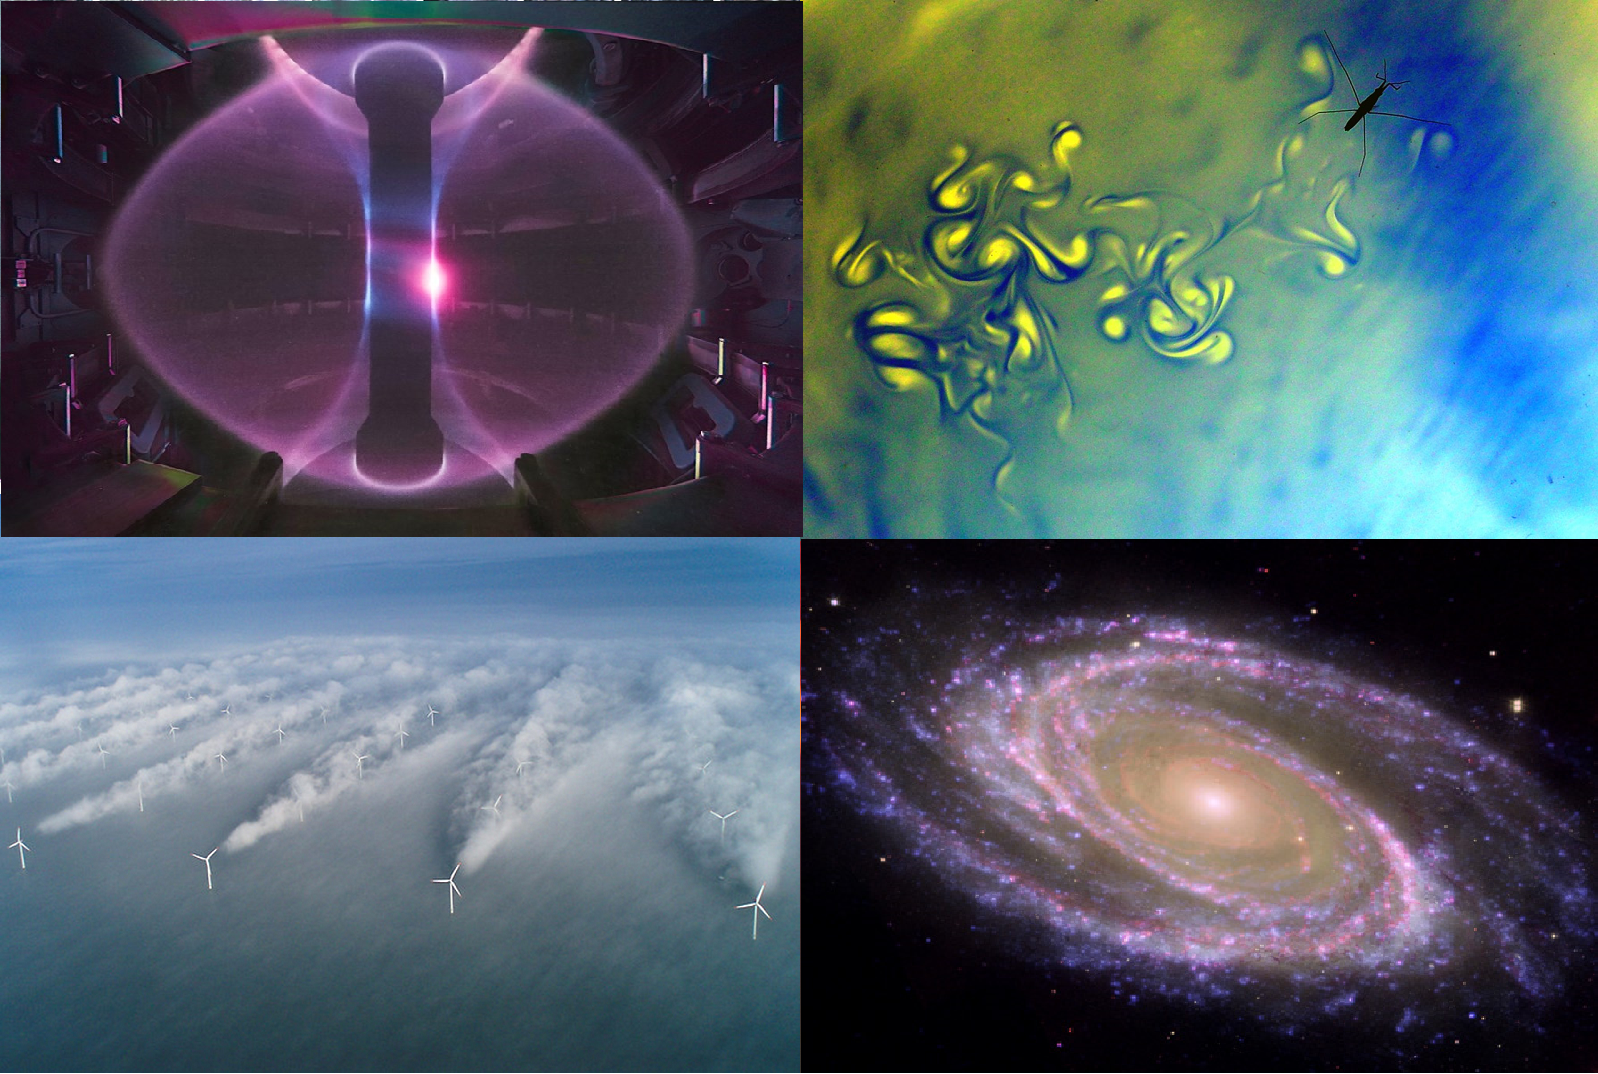
\includegraphics[width=4.3in]{Composite2.PNG}\footnotemark
\end{figure}
}


\subsection{What is an Integral Equation?} 
\frame{\frametitle{\subsecname}
\begin{itemize}
\item Integral equations one way of solving PDEs, involve operations like solution of integral equations:
\be \int_\Omega K(\mathbf{x},\mathbf{y}) \, \sigma(\mathbf{y}) \,d\mathbf{y} = f(\mathbf{x})\ee
($K$ is a kernel function and $\sigma(\mathbf{y})$ unknown)
\item Or evaluation of integrals:
\be \phi(\mathbf{x}) = \int_\Omega K(\mathbf{x},\mathbf{y}) \, \sigma(\mathbf{y}) \,d\mathbf{y} \ee

\item Central idea: solution of PDE sum of "fundamental solutions" $G$ that solve PDE for point source (in the weak sense):
\be \mathcal{L}G(x,y) = \delta(y-x) \ee
$\mathcal{L}$ is linear differential operator associated with PDE, $G$ the \textit{Green's function}, $\delta$ Dirac delta.
\end{itemize}
}

\subsection{How are They Useful?} 
\frame{\frametitle{\subsecname}
\begin{itemize}
\item Example: Poisson equation:
\be \nabla^2 \phi = f \ee
\item Solution given by evaluating:
\be \phi(\mathbf{x}) = \int_\Omega G(\mathbf{x},\mathbf{y}) \, f(\mathbf{y}) \,d\mathbf{y} \hskip 0.3in G(\mathbf{x},\mathbf{y}) = \frac{1}{4 \pi |\mathbf{x}-\mathbf{y}|} \ee

\item Integral equation methods evaluated with FMM competitive efficiency-wise with other approaches\footnotemark, and have excellent conditioning
\item Evaluation of the integrals can pose challenges
\end{itemize}
}

\subsection{Numerical Integral Evaluation}
\frame{\frametitle{\subsecname}
%\vskip -0.1in
%\begin{equation*} \int_\Omega K(\mathbf{x},\mathbf{y}) \, \sigma(\mathbf{y}) \,d\mathbf{y} \end{equation*}
%\vskip -0.1in
\begin{itemize}
\item Issue: Gaussian quadrature assumes integrand approximated well by polynomials
\item Poor assumption since $K$ is usually singular or near singular
\item Consider common singularity, quadrature converges\footnotemark \,slowly:
\vskip -0.2in
\be \hskip -0.2in y \in [-1,1] , \,\, I(y)=\int_{-1}^1 |x-y|^{-\delta} dx \, , \,\,\, |I-I_n| < \mathcal{O}(n^{-1 + \delta}) \ee
\item Approaches include: product integration rules\footnotemark; compute offline, weights that exactly integrate up to a polynomial order
\item Transformation of the integral\footnotemark (e.g. to a semi-infinite domain), causes singularity to vanish
\item Adaptive quadrature; adaptively divide domain based on error estimate, compute on each subdomain
\end{itemize}
}

\subsection{More General Scheme for Unstructured Meshes} 
\frame{\frametitle{\subsecname}
\begin{itemize}
\item Mentioned approaches lack generality: tied to specific integrand and/or for unmapped/structured meshes
\item We want a high-order general purpose quadrature method that works for unstructured meshes and complex geometries
\item For inspiration look to QBX (Quadrature by Expansion)\footnotemark: high-order, geometric flexibility
\end{itemize}
\begin{figure}
\centering
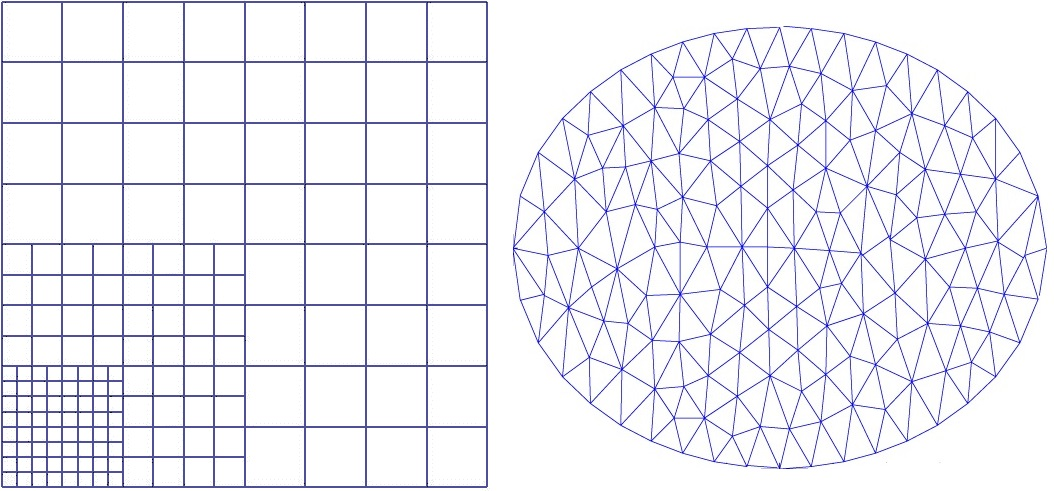
\includegraphics[width=3in]{blob.jpg}\footnotemark
\end{figure}
}

\section{Methodology}
\subsection{QBX for Volume Potentials} 
\frame{\frametitle{\textbf{\secname}: \subsecname}
\begin{itemize}
\item Volume potential share similarities to layer potentials
\item Same main challenge: devising quadrature to handle singularity
\item Take same approach: QBX
\item But where do we put our expansion center, fictitious dimension?
\item Off-surface: layer potential physically defined, off-volume has no requirements
\end{itemize}
\begin{figure}
\centering
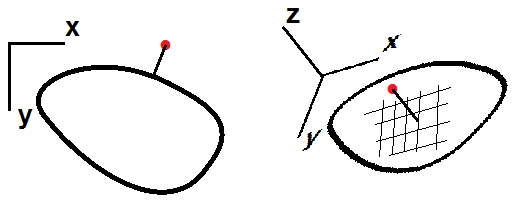
\includegraphics[width=4in]{LayVol.PNG}
\end{figure}
}

\subsection{Trial Scheme} 
\frame{\frametitle{\subsecname}
\begin{itemize}
\item Absent any compelling choice for off-volume potential, choose obvious one:
\item Consider 3D Poisson scheme: approximate $G = 1/r$ kernel with $\hat{G} = 1/\sqrt{r^2+a^2}$
\item Effectively $a$ parameter is the distance from expansion center to eval point in the fictitious dimension, and kernel is no longer singular
\item Choose a ``good'' $a$ so the kernel is smooth and take QBX approach of evaluating Taylor expansion of de-singularized kernel back at desired eval point
\end{itemize} 
}

\subsection{Is trial scheme high-order?} 
\frame{\frametitle{\subsecname}
\begin{itemize}
\item No, in fact seems to be limited to second order regardless of expansion order.
\item Consider example results in figure below for 6th order expansion.
\item Why only second order?
\end{itemize}
\begin{figure}
\centering
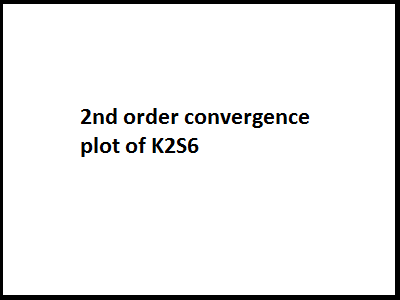
\includegraphics[width=3in]{2orderK2.PNG}
\end{figure}
}

\subsection{Preliminary Error Analysis} 
\frame{\frametitle{\subsecname}
\begin{itemize}
\item We would like to examine the error \\ $\epsilon = |$Exact potential - QBX computed potential$|$\\ and it's dependence on $a$
\item Call $T_k$ the k-th order Taylor series expansion of $\hat{G}$ about $d$ and evaluated at $a=0$: $$T_k(r,d) = \sum^k_{n=0}\frac{(-d)^n}{n!}\hat{G}^{(n)}(r,d)$$
\item So our error is: $$\epsilon_k = \int_\Omega G(r) \sigma(r) \, dr - \int_\Omega T_k(r,d) \sigma(r) \, dr$$
\item This form seems complicated to inspect, is there a way to avoid the integrals and factor out the density?
\end{itemize} 
}

\subsection{Error in Fourier Space} 
\frame{\frametitle{\subsecname}
\begin{itemize}
\item Consider the action of the Fourier transform on the error:
$$\mathcal{F}[\epsilon] = \mathcal{F}\left[ \int G \, \sigma \, dr \right] - \mathcal{F}\left[ \int T_k \, \sigma \, dr \right]$$
and by the convolution theorem:
$$= \mathcal{F}[G] \, \mathcal{F}[\sigma] - \mathcal{F}[T_k]\,\mathcal{F}[\sigma] = \mathcal{F}[\sigma] \left(\mathcal{F}[G] - \mathcal{F}[T_k]\right)  $$
$$\mathcal{F}[T_k] = \sum_{n=0}^k \frac{(-d)^n}{n!} \mathcal{F}[\hat{G}^{(n)}(r,d)]$$
\item This looks more reasonable, let's examine the behavior of $\mathcal{F}[G] - \mathcal{F}[T_k]$ with respect to $d$.
\end{itemize} 
}

\subsection{Fourier Transform Particulars} 
\frame{\frametitle{\subsecname}
\begin{itemize}
\item Need 3D Fourier transform; both $G$ and $T$ are radially symmetric, so simplifications can be made: transforms can be given in terms of the scalar $k$ in Fourier space.
\item It is known that $\mathcal{F}[1/r] = 1/\pi k^2$
\item With some work one can show:
$$\mathcal{F}[\frac{1}{\sqrt{r^2+a^2}}] = \frac{2 a}{k}K_1(2 \pi a k)$$
where $K_n(x)$ is the modified Bessel function of second kind
\item Reduces to expected form for $\lim_{a \to 0} \frac{2 a}{k}K_1(2 \pi a k) = 1/\pi k^2$
\item Without concerning ourselves with details, in general we find:
$$\mathcal{F}[T_k] = \sum_{n=-1}^k C_n \, d^{n+2} \, k^nK_n(2 \pi k d)$$
\end{itemize} 
}

\subsection{Examination of Error}
\frame{\frametitle{\subsecname}
\begin{itemize}
\item k dependence tells us how well the expansion preserves low vs high modes in real space (in figure below $d=0.2$)
\item Taylor expansion of $\mathcal{F} [T_5]$ wrt $d$ about 0:
$$ \frac{1}{\pi k^2} +\frac{\pi d^2}{10}+ \frac{1}{20} \pi ^3 d^4 k^2+ \mathcal{O}(d^6)$$
\end{itemize}
\vskip -0.1in
\begin{figure}
\centering
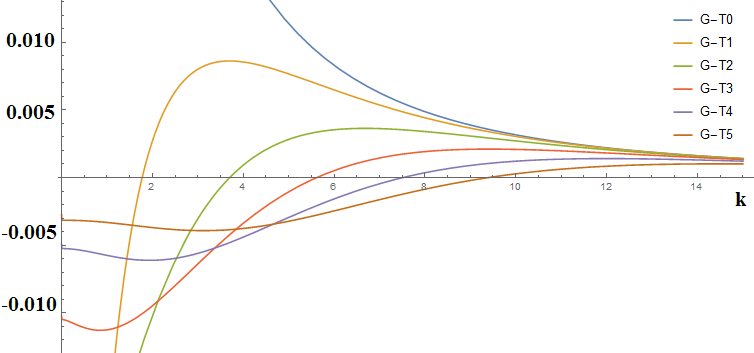
\includegraphics[width=4.5in]{G-Tmod.PNG}
\end{figure}
}

\subsection{Cause: Approximation Error}
\frame{\frametitle{\subsecname}
\begin{itemize}
\item It seems there is some additional approximation error that limits convergence, truncation error from Taylor series not the issue
\item We replaced Green's function with de-singularized approximation, what does approximate kernel correspond to?
\item Remember that for our Laplace equation
\be \nabla^2 G(x,y) = \delta(y-x) \ee
\item However our de-singularized Green's function doesn't satisfy this, instead of solving for a point source it solves for a blob source: $\zeta$
\be \nabla^2 \hat{G}(x,y) = \zeta(y-x) \ee
\end{itemize}
}

\subsection{Dirac Delta Approximation and Moment Conditions}
\frame{\frametitle{\subsecname}
\begin{itemize}
\item The quality of our Green's function approximation then depends upon the quality of our Dirac delta approximation from our choice of a blob
\item The order of convergence of this approximation can be shown\footnotemark$^,$\footnotemark \, to depend upon the \textit{moment conditions}, where for a $s$ order accurate approximation we require:

\be \int \zeta(\mathbf{x}) \, d\mathbf{x} = 1\ee
\be \int \mathbf{x}^{\mathbf{i}} \, \zeta(\mathbf{x}) \, d\mathbf{x} = 0 \, , \, |\mathbf{i}|<s-1\ee
\be \int \mathbf{x}^s \, \zeta(\mathbf{x}) \, d\mathbf{x} < \infty \ee

\end{itemize}
}

\subsection{High Order De-singularized Kernels}
\frame{\frametitle{\subsecname}
\begin{itemize}
\item We can see that $1/\sqrt{r^2 + a^2}$ is actually 0th order approximation (the third condition isn't totally satisfied for $s=2$)
\item This approximation error in turn bounds our overall error and limits convergence rate to at best 2nd order
\item Why better convergence than expected from kernel? Postulated QBX expansion satisfies moment conditions for $s=2$, remains to be verified
\item Possible to construct higher-order kernels by satisfying moment conditions\footnotemark for larger $s$
\item For example consider the 2nd order kernel (i.e. satisfies moment conditions for $s=2$: 
\be \zeta = \frac{15/2}{(r^2 + a^2)^{7/2}} \rightarrow  \hat{G} = \frac{r^2 + \frac{3}{2} a^2}{(r^2 + a^2)^{3/2}}\ee

\end{itemize}

}

\subsection{Fourier Space Error Analysis of High Order Kernels}
\frame{\frametitle{\subsecname}
\begin{itemize}
\item Define $T_{s,k}$ to be similar to our $T_k$ from before, but now for $\hat{G}_s$ the $s$th order algebraic approximate kernel
\item We can examine again the error in our computed integral in Fourier space, but now for our higher order kernel
\item We find that in general:
\be \hskip -0.5in  \mathcal{F}[T_{s,k}] =  \frac{2}{(\frac{s}{2})!}d^n k^{n - 2} \pi^{n - 1} K_{\frac{s}{2} +1}(2 \pi k d) \,+ \!\!\!\! \sum_{n=\frac{s}{2} - 1}^k \!\!\! C_n \, d^{n+2} \, k^n \pi^{n+1} K_n(2 \pi k d) \ee
\item For example, consider the Taylor expansion of higher order kernels wrt $d$ about 0:
$$ \hskip -0.3in \mathcal{F} [T_{2,5}] \rightarrow \frac{1}{\pi k^2} +\frac{k^2 \pi^3 d^4}{20}+ \mathcal{O}(d^6) \,\, , \,\, \mathcal{F} [T_{4,7}] \rightarrow \frac{1}{\pi k^2} +\frac{k^4 \pi^5 d^6}{252}+ \mathcal{O}(d^8)$$
\end{itemize}
}

\section{Results}
\subsection{Test Setup} 
\frame{\frametitle{\textbf{\secname}: \subsecname}
\begin{itemize}
\item Theoretical computed convergence rates were verified empirically
\item Integral evaluated for 3D Laplace Green's function with constant density in domain $[-0.5, 0.5] \times [-0.5, 0.5] \times [-0.5, 0.5]$
\item Possible to compute exact analytical expression for any target in domain
\item Domain split into cube elements and tensor product Gauss-Legendre quadrature of varying order was used
\item Computed result compared with exact result to determine error, and with $h$ refinement the order of convergence
\end{itemize}
}

\subsection{Required Minimum Quadrature Order}
\frame{\frametitle{\subsecname}
\begin{itemize}
\item Accuracy of result dependent on choice of quadrature order $q$ and value chosen for $d$
\item Min required quadrature order to accurately evaluate integral, smaller $d$ less smooth kernel and higher required $q$
\item Past min $q$, error dominated by truncation error in expansion
\begin{figure}
\centering
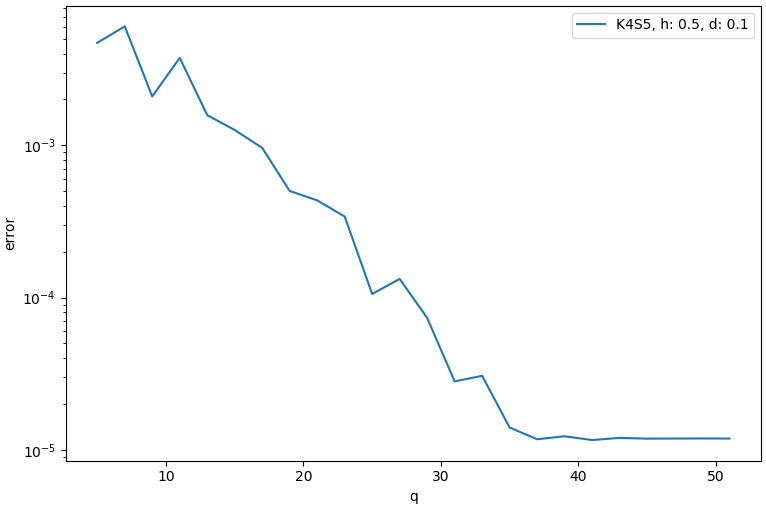
\includegraphics[width=3in]{minqd.PNG}
\end{figure}
\end{itemize}
}

\subsection{Observed Convergence}
\frame{\frametitle{\subsecname}
\begin{figure}
\centering
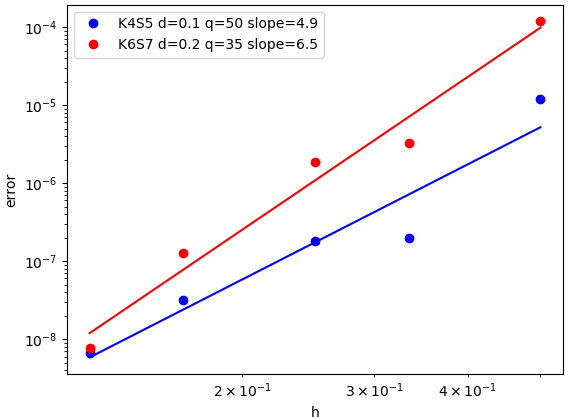
\includegraphics[width=4.5in]{convg12.PNG}
\end{figure}
}

\subsection{Quadrature Error Bounds}
\frame{\frametitle{\subsecname}
\begin{itemize}
\item Content dependent on how far I get with TV error estimate by Thurs night
\item Explanation of bounding quadrature error\footnotemark in terms of
\item Analytic continuability
\item and Total Variation (TV)
\end{itemize}
}

\subsection{Rough TV Bound Behavior}
\frame{\frametitle{\subsecname}
\begin{itemize}
\item Relate bound on required $q$ and $d$, and behavior wrt $h$ refinement

\end{itemize}
}

\subsection{Observed Error Correctly Bounded by Estimate}
\frame{\frametitle{\subsecname}
\begin{itemize}
\item Hopefully show here that observed \textit{quadrature error} (not \textit{total error}) is properly bounded by the TV estimate

\end{itemize}
}

\section{Conclusion}
\frame{\frametitle{\textbf{\secname}}
\begin{itemize}
\item 
\item 
\item 
\item 
\item 
\end{itemize}
}

\section{References}
\frame{\frametitle{\textbf{\secname}}
\begin{itemize}
\tiny
\item [1]  iter.org/sci/plasmaconfinement, www-math.mit.edu/dhu/Striderweb/striderweb.html, noaanews.noaa.gov/stories2011/20110426\_windwakes.html, nasa.gov/spitzer-20070604.html
\item [2] Gholami, Amir, et al. "FFT, FMM, or Multigrid? A comparative Study of State-Of-the-Art Poisson Solvers for Uniform and Nonuniform Grids in the Unit Cube." SIAM Journal on Scientific Computing 38.3 (2016): C280-C306.
\item [3] Lubinsky, Rabinowitz. "Rates of convergence of Gaussian quadrature for singular integrands." Mathematics of Computation 43.167 (1984): 219-242.
\item [4] Strain. Fast adaptive 2D vortex methods. Journal of Computational Physics 132.1 (1997): 108-122.
\item [5] Huybrechs, Cools. "On generalized Gaussian quadrature rules for singular and nearly singular integrals." SIAM Journal on Numerical Analysis 47.1 (2009): 719-739.
\item [6] Klöckner, et al. "Quadrature by expansion: A new method for the evaluation of layer potentials." Journal of Computational Physics 252 (2013): 332-349.
\item [7] http://www.ae.metu.edu.tr/tuncer/ae546/prj/delaundo/files/small0012.gif
\item [8] Cottet, Koumoutsakos. Vortex methods: theory and practice. Cambridge university press, 2000.
\item [9] Liu, Mori. "Properties of discrete delta functions and local convergence of the immersed boundary method." SIAM Journal on Numerical Analysis 50.6 (2012): 2986-3015.
\item [10] Winckelmans, Leonard. "Contributions to vortex particle methods for the computation of three-dimensional incompressible unsteady flows." Journal of Computational Physics 109.2 (1993): 247-273.
\item [11] Trefethen, Lloyd N. Approximation Theory and Approximation Practice. Vol. 128. Siam, 2013.
\end{itemize}
}

\end{document}